% Standalone figure: LM training loss (BPE vs MorphBPE), split into two
% panels by model size -- mirrors the source paper's own Figure 3 (small
% vs. large model, side by side), but unlike that figure, our two panels
% don't share the same language set: Cree and Guarani only exist at the
% smaller (~1.3M-param) scale, Inuktitut only at the larger (~3.1M-param)
% scale (see report/writeup.md Section 4 for why). Splitting by panel
% keeps each language's curve next to only the others trained at the same
% scale, so the "don't compare absolute values across panels" caveat is
% visible in the layout itself, not just stated in the caption.
%
% Color: blue = Cree, orange = Inuktitut, bluish green = Guarani (Okabe-Ito
% categorical triple -- validated colorblind-safe combination). Linestyle
% carries the second dimension (dashed = BPE, solid = MorphBPE).
\documentclass[tikz]{standalone}
\usepackage{times}
\usepackage{pgfplots}
\pgfplotsset{compat=1.18}
\usepgfplotslibrary{groupplots}

\definecolor{seriesCree}{HTML}{2A78D6}
\definecolor{seriesInuktitut}{HTML}{EB6834}
\definecolor{seriesGuarani}{HTML}{009E73}
\definecolor{gridcolor}{HTML}{E1E0D9}
\definecolor{axiscolor}{HTML}{C3C2B7}
\definecolor{mutedtext}{HTML}{898781}
\definecolor{primaryink}{HTML}{0B0B0B}

\begin{document}
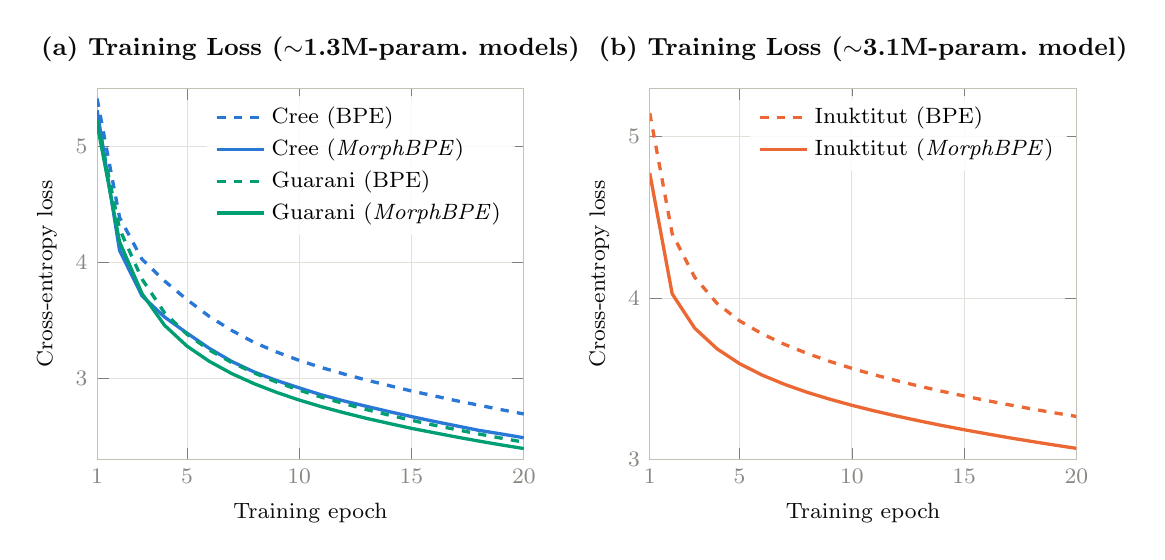
\begin{tikzpicture}
\begin{groupplot}[
    group style={
        group size=2 by 1,
        horizontal sep=1.6cm,
    },
    width=7cm, height=6.3cm,
    xlabel={Training epoch},
    ylabel={Cross-entropy loss},
    xmin=1, xmax=20,
    xtick={1,5,10,15,20},
    grid=major,
    grid style={gridcolor, line width=0.3pt},
    axis line style={axiscolor},
    tick label style={color=mutedtext, font=\footnotesize},
    label style={color=primaryink, font=\footnotesize},
    title style={color=primaryink, font=\bfseries\small},
    legend style={
        font=\footnotesize,
        draw=none,
        fill=white,
        fill opacity=0.85,
        text opacity=1,
        at={(0.98,0.98)},
        anchor=north east,
    },
    legend cell align=left,
    every axis plot/.append style={line width=1.2pt, mark=none},
]

\nextgroupplot[title={(a) Training Loss ($\sim$1.3M-param.\ models)}, ymin=2.3, ymax=5.5]
\addplot[seriesCree, dashed] coordinates {
    (1,5.409744389851888) (2,4.386526346206665) (3,4.026913932959238)
    (4,3.839942232767741) (5,3.679182934761047) (6,3.533221205075582)
    (7,3.4127057075500487) (8,3.3093050122261047) (9,3.227153480052948)
    (10,3.155119327704112) (11,3.093248935540517) (12,3.0376282731691995)
    (13,2.985764479637146) (14,2.9383687456448873) (15,2.8919909795125327)
    (16,2.85012233654658) (17,2.8080217401186625) (18,2.7696027636528013)
    (19,2.730829155445099) (20,2.6938249349594114)
};
\addlegendentry{Cree (BPE)}

\addplot[seriesCree, solid] coordinates {
    (1,5.309244427314171) (2,4.10192165007958) (3,3.7109610374157245)
    (4,3.529307277386005) (5,3.390667618238009) (6,3.258465106670673)
    (7,3.1455732895777775) (8,3.05503328029926) (9,2.981681966781616)
    (10,2.9186128579653228) (11,2.857948974462656) (12,2.8056417281811052)
    (13,2.7595270230219913) (14,2.7142072897690994) (15,2.67128178523137)
    (16,2.630489947245671) (17,2.5915081427647517) (18,2.5529855508070725)
    (19,2.5217796949239877) (20,2.4891653501070463)
};
\addlegendentry{Cree (\textit{MorphBPE})}

\addplot[seriesGuarani, dashed] coordinates {
    (1,5.224725457659939) (2,4.286658115554274) (3,3.8551399467284218)
    (4,3.5652930987508675) (5,3.3806605328593338) (6,3.2443483335930003)
    (7,3.1365973395213746) (8,3.046502269150918) (9,2.9679102029716757)
    (10,2.899291479796694) (11,2.8378573812936483) (12,2.7830903603319537)
    (13,2.7316647872590183) (14,2.6840884298609016) (15,2.639471821617662)
    (16,2.597696984023379) (17,2.5590318702814874) (18,2.521374328094616)
    (19,2.4855177203814187) (20,2.451333114975377)
};
\addlegendentry{Guarani (BPE)}

\addplot[seriesGuarani, solid] coordinates {
    (1,5.19164489877635) (2,4.176312266752638) (3,3.730721972111998)
    (4,3.458076004324288) (5,3.278673775237182) (6,3.1468275590189574)
    (7,3.0413718501041673) (8,2.954082681187268) (9,2.87938434810474)
    (10,2.8138099651912163) (11,2.75597928515796) (12,2.703983799136918)
    (13,2.655852682631591) (14,2.612422853708267) (15,2.5699227945557954)
    (16,2.5326147233617715) (17,2.4955053041721214) (18,2.460487581532577)
    (19,2.4272499156409295) (20,2.3962494926205995)
};
\addlegendentry{Guarani (\textit{MorphBPE})}

\nextgroupplot[title={(b) Training Loss ($\sim$3.1M-param.\ model)}, ymin=3.0, ymax=5.3]
\addplot[seriesInuktitut, dashed] coordinates {
    (1,5.145976681575597) (2,4.398943669823224) (3,4.129752070980528)
    (4,3.967109422941198) (5,3.85960052912109) (6,3.7795338192461436)
    (7,3.7142577413953104) (8,3.6583696104903334) (9,3.6094431020512885)
    (10,3.565575699939906) (11,3.52565293297218) (12,3.4890820764678288)
    (13,3.4554464557089166) (14,3.4240319392143874) (15,3.3942550241266334)
    (16,3.3662945023454487) (17,3.340064173794486) (18,3.31474922701082)
    (19,3.2904876078153076) (20,3.2679009598487387)
};
\addlegendentry{Inuktitut (BPE)}

\addplot[seriesInuktitut, solid] coordinates {
    (1,4.774372222896734) (2,4.026608575453351) (3,3.8146111439424186)
    (4,3.6861443357293924) (5,3.5945940554884914) (6,3.524129667309535)
    (7,3.466764019411111) (8,3.4176540975945566) (9,3.375257618932459)
    (10,3.3369444989289443) (11,3.302196471825999) (12,3.270154822935651)
    (13,3.2403360972125603) (14,3.2121411873990255) (15,3.18564347247035)
    (16,3.160443723601783) (17,3.1360984253174737) (18,3.1132796379886676)
    (19,3.0913377601371175) (20,3.0703356252306375)
};
\addlegendentry{Inuktitut (\textit{MorphBPE})}

\end{groupplot}
\end{tikzpicture}
\end{document}
